\documentclass{edm_template}
\usepackage{cite}
\usepackage{amsmath,amssymb,amsfonts}
\usepackage{algorithmic}
\usepackage{graphicx}
\usepackage{textcomp}
\usepackage{xcolor}
\usepackage{algorithm}
\usepackage{algorithmic}
\usepackage{enumerate}
\usepackage[english]{babel}
\usepackage{blindtext}
\usepackage{indentfirst}
\usepackage{latexsym}
\usepackage{array}
\usepackage{graphicx}
%\usepackage{subcaption}
\usepackage{fixltx2e}
\usepackage{dblfloatfix}

% \def\BibTeX{{\rm B\kern-.05em{\sc i\kern-.025em b}\kern-.08em
%     T\kern-.1667em\lower.7ex\hbox{E}\kern-.125emX}}

% \columnsep 0.2in
% \usepackage{changes}
% 	\definechangesauthor[name={Per cusse}, color=orange]{per}
% 	\setremarkmarkup{(#2)}
\begin{document}

% \title{Exercises Sequence Recommendation based on exercise-Level Knowledge Tracing}
% \title{Accuratly Tracking and Improving Human Learning with Deep Reinforcement Learning}
% \title{Accuratly Student Tracing and Exercise Recommendation with Deep Learning in a Online Self-Learning System}

\title{Concept-Aware Deep Knowledge Tracing and Exercise Recommendation in an Online Learning System}

% \numberofauthors{3}
% \author{
% 	\alignauthor
% 	Fangzhe Ai, Yishuai Chen, Yuchun Guo, Yongxiang Zhao\\
% 	\affaddr{School of Electronics and Information Engineering}
% 	\affaddr{Beijing Jiaotong University}
% 	\email{17125001, yschen, ychguo, yxzhao@bjtu.edu.cn}
% 	\alignauthor
% 	Guangyan Wang\\
% 	\affaddr{College of Education}\\
% 	\affaddr{Hebei University}
% 	\email{gywang@163.com}
% 	\alignauthor
% 	Guowei Fu\\
% 	\affaddr{TAL Education Group Inc.}\\
% 	\affaddr{Beijing, China, 100080}
% 	\email{fuguowei@100tal.com}
% }
\numberofauthors{7}
\author{
	\alignauthor
    %anonymous for review\\
	Fangzhe Ai\\
	\affaddr{School of Electronics and Information Engineering}
	\affaddr{Beijing Jiaotong University}
	\email{17125001@bjtu.edu.cn}
	\alignauthor
	Yishuai Chen\\
	\affaddr{School of Electronics and Information Engineering}
	\affaddr{Beijing Jiaotong University}
	\email{yschen@bjtu.edu.cn}
	\alignauthor
	Yuchun Guo\\
	\affaddr{School of Electronics and Information Engineering}
	\affaddr{Beijing Jiaotong University}
	\email{ycguo@bjtu.edu.cn}
	\and
	\alignauthor
	Yongxiang Zhao\\
	\affaddr{School of Electronics and Information Engineering}
	\affaddr{Beijing Jiaotong University}
	\email{yxzhao@bjtu.edu.cn}
	\alignauthor
	Guowei Fu\\
	\affaddr{TAL Education Group Inc.}\\
	\affaddr{Beijing, China, 100080}
	\email{fuguowei@100tal.com}
	\alignauthor
	Zhenzhu Wang\\
	\affaddr{School of Electronics and Information Engineering}\\
	\affaddr{Beijing Jiaotong University}
	\email{18120144@bjtu.edu.cn}
}
% \author{\IEEEauthorblockN{Mengfei Feng, Yishuai Chen, Junfeng Li, Fangzhe Ai, Yuchun Guo, Yongxiang Zhao}
% \IEEEauthorblockA{\textit{School of Electronics and Information Engineering} \\
% \textit{Beijing Jiaotong University}\\
% Beijing, China \\
% \{17120052,yschen,15120206,17125001,ychguo,yxzhao\}@bjtu.edu.cn}
% }

\additionalauthors{Additional authors: 
Guangyan Wang (College of Education, Hebei University,
email: {\texttt{gywang@163.com}}).}

\maketitle


\begin{abstract}

Personalized education systems recommend learning contents to students based on their capacity to accelerate their learning. 
% For instance, contents which are too easy or too hard for students should be avoided. Personalized education based on machine learning can serve more learners than one-on-one human tutoring.
This paper proposes a personalized exercise recommendation system for online self-directed learning. We first improve the performance of knowledge tracing models. Existing deep knowledge tracing models, such as 
% including Deep Knowledge Tracing (DKT) and 
Dynamic Key-Value Memory Network (DKVMN), ignore exercises' concept tags, which are usually available in tutoring systems. We modify DKVMN to design its memory structure based on the course's concept list, and explicitly consider the exercise-concept mapping relationship during students' knowledge tracing. We evaluated the model on the 5th grade students' math exercising dataset in TAL, one of the biggest education groups in China, and found that our model has higher performance than existing models. We also enhance the DKVMN model to support more input features and obtain higher performance.
Second, we use the model to build a student simulator, and use it to train an exercise recommendation policy with deep reinforcement learning. 
% Experimental results show that the policy helps students have higher knowledge level after solving fewer exercises than the heuristic policy does. 
% Then, we build a student simulator with our modified model to train an exercises recommendation policy that uses model-free reinforcement learning with neural network. 
Experimental results show that our policy achieves better performance then existing heuristic policy in terms of maximizing the students' knowledge level.
To the best of our knowledge, this is the first time that deep reinforcement learning has been applied to personalized mathematic exercise recommendation.
	% students have higher probability of getting exercises correct after solving fewer problems. 

    % Based on the data, we also measured and analyzed the dependency of various student behavior features such as duration of finishing exercises.
    % Inspired by DKT and DKVMN, in this paper, we propose a deep knowledge tracing model
	% Knowledge tracing is to model student's knowledge status through student's exercises performance data. Personalized exercises recommendation based on student's own knowledge status, helps student to quickly master and apply knowledge. At present, online education has become an important part during the student learning process. Students study on the online education system, at the same time, the system also records various information during the student's learning process. However, this information is not fully used for student's knowledge tracing, and the exercises recommendation is mostly based on remedial policy, without considering profit of the entire exercise sequence. Therefore, we first measure and analyze the student learning log of an online exercise system, improve the performance of the knowledge tracing model by rich features such as multi-level knowledge concepts and duration of finishing exercises. Then, we build a student simulator by the modified knowledge tracing model, and optimize the exercise recommendation policy by reinforcement learning. Experiment results on real data show that the obtained policy takes the dependence relationship of different knowledge concepts into account when making recommendations, thus improving the knowledge level of the students faster.
\end{abstract}

\section{Introduction}

% Education mainly includes two main links: teaching interaction and practice. Knowledge is presented to students through instructional interactions, and students then enhance their mastery of knowledge by a series of exercises. However, because of the limited educational resources, teachers do not have the energy and time to customize the exercise program for each student.

Online self-directed learning systems, such as Massive Open Online Courses (MOOCs), are prevailing. These systems, however, assign same exercises to all students, which is inefficient. For comparison, personalized exercises recommendation can improve the efficiency of students' learning. In this paper, we propose a personalized exercise recommendation system for an online self-directed learning service. The system consists of two parts:
\begin{itemize}
	\item A student knowledge tracing model, which traces a student's knowledge state and predicts whether or not she can finish the exercise correctly.
	\item A personalized exercise recommendation policy which recommends appropriate exercises to students to accelerate her learning process.
\end{itemize}

Existing deep knowledge tracing models \cite{dkt,dkvmn} ignore exercises' knowledge concept properties, which are usually available in tutoring systems. For comparison,
% Traditional representation method of exercises' concept tags, however, cannot bring considerable performance gain to the model.
% The traditional method represents a knowledge concept by its embedding and then concatenate it with the embedding of the exercise cannot bring considerable performance gain to the model. In this paper, we evaluate this method and prove this result.
in this paper, we propose a concept-aware deep knowledge tracing model. The model is inspired by Dynamic Key-Value Memory Network (DKVMN) model \cite{dkvmn}. DKVMN model has a static matrix called \textit{key} which stores the latent knowledge concepts and a dynamic matrix called \textit{value} which stores a student's concept mastery levels. The model computes the correlation between an exercise and the latent concepts in the \textit{key}, and then uses it to read the student's concept mastery levels in the \textit{value}, and predict whether the student will finish the exercise correctly. 
% After the student completes the exercise, the model will use the same correlation weight to update the related \textit{value} states. 
We improve the DKVMN model as follows: 1) we design its memory structure based on the course's concept list and explicitly consider the exercise-concept mapping relationship during students' knowledge tracing. 2) We enhance it to support more input features, including exercise difficulty, stages, and student practice time. We evaluated the model on the 5th grade students' math exercising dataset in TAL, and found that our model has higher performance than existing deep knowledge tracing models.

In terms of personalized exercise recommendation policy, most of existing algorithms are heuristic, e.g., exercises which are too easy or too hard for a student should be avoided. These algorithms may be not optimal, as they only consider the short-term reward.
 % resulting that students can't make greater progress. For example, basic exercises are more meaningful than difficult exercises to the weaker students although they happened to answer the difficult exercise correctly.
 % e.g., exercises which are too easy or too hard for the student should be avoided.
% Existing Markov Decision Process based exercise recommendation algorithm \cite{dkt} only consider short-term gains of the recommended exercises and the performance may be not optimal. overall benefits of a complete sequence of recommended exercises.
In this paper, we build a student simulator with our concept-aware deep knowledge tracing model, and then use it to train a flexible and scalable personalized exercise recommendation policy with deep reinforcement learning, which considers long-term reward of recommended items.

% For this goad, we first use the model to built a student simulator, and use the simulator to train an exercise recommendation policy using deep reinforcement learning. Experimental results shown that with the help of the policy, students have higher predicted knowledge after solving fewer problems. To the best of our knowledge, this is the first time that deep reinforcement learning is applied for personalized mathematic exercise recommendation.

% , but they use the single knowledge concept label instead of the exercise tag for knowledge tracing, ignoring multi-level knowledge concepts information and the behavior information such as the time of answerring exercise, can not better trace the status of knowledge concepts.


% Intelligent Practice System (IPS), etc.,

% Therefore, in this paper, we first measure and evaluate the correlation between these student behaviors characteristics and the answering status of the exercises, and then design a new deep tracing model considering these information. The model's AUC is 73.9\%, which is 1.9\% higher than 72.0\% of the DKT and DKVMN. Such a result proves that the consideration of the knowledge concept structure is beneficial for the deep tracing model. Based on the model, we built a student simulator and evaluate the performance of exercise recommendation policy obtained by reinforcement learning. Experimental results shown that that with the help of reinforement learning, the students can obtain higher average score. To the best of our knowledge, this is the first time that reinforcement leanring is applied to improve the exercise recommendation.

% improve knowledge tracing model through other features of the exercise, such as multi-level knowledge concepts. Assess the impact of different features on the knowledge tracing model to better utilize multi-level knowledge concepts and student behavior characteristics for knowledge tracing.
% We model the student's learning process as the Partially Observable Markov Decision Process(POMDP), optimize the policy by TRPO algorithm. Analyze and compare the knowledge status changing along the exercises sequence recommended by expectimax algorithm and our recommendation algorithm.
In summary, 
% in this paper, we present our design and evaluation results of a personalized exercise recommendation system for an online self-directed learning service. 
the main contributions of this paper are two folds:
\begin{itemize}
\item
We propose a new exercise-level deep knowledge tracing model whose structure is built based on the course's concept list, and the exercise-concept mapping relationships are utilized during students' knowledge tracing. The model supports more input features and obtains higher performance compared with existing models.
\item
We propose an exercises recommendation algorithm which uses model-free reinforcement learning with neural network function approximation to learn an exercise recommendation policy. The policy directly operates on raw observations of a student's exercise history. Experimental results show that our policy achieves better performance than existing heuristic policy in terms of maximizing students' knowledge level.

% \item
% We proposed a new exercise-level deep knowledge tracing model whose structure is built based on the course's concept list, and the exercise-concept mapping relationship are utilized during students' knowledge tracing.
% % We also measured and analyzed the dependency of various student behavior features such as the gate where student is doing exercises, and duration of finishing exercises, and included them as the input of our model. We evaluated the model on a large-scale K-12 student math exercising dataset in TAL, one of the biggest education group in China. The
% Experimental results show that our model obtains an area under the curve (AUC) of 0.724 which is a notable improvement over the performance of the state-of-art DKVMN model (AUC = 0.712), especially when compared to the small improvement DKVMN provided over the DKT baseline (AUC = 0.711).
% % 's area under the curve (AUC) is (0.728-0.712)/0.712 = 2.25\% , and 0.7281.9\% higher than the LSTM-based and DKVMN deep knowledge tracing (AUC 0.712, and 0.728).
% % We also enhance the DKVMN model to support more input features and obtain higher performance.
% % Such a result validates that the consideration of the knowledge concept structure is beneficial for the deep tracing model.
% We also proved that the consideration of exercises' difficulty, level, and duration of a student's exercising can further improve the model's performance. For example, our model with difficulty of exercise as feature has AUC 0.726.

% \item
% We built a student simulator with our knowledge tracing model, and used it to train an exercise recommendation policy with deep reinforcement learning algorithm. Experimental results shown that with the help of the policy, students have higher probability of getting exercises correct after solving fewer problems. 
% To the best of our knowledge, this is the first time that deep reinforcement learning is applied for personalized mathematic exercise recommendation.

% and evaluate the performance of exercise recommendation policy obtained by reinforcement learning. Experimental results shown that with the help of reinforcement learning, students have higher predicted knowledge after solving fewer problems. To the best of our knowledge, this is the first time that deep reinforcement learning is applied to improve mathematics exercise recommendation.
% Build a student simulator by knowledge tracing, design a personalized exercises recommendation framework by reinforcement learning which has better performance of policy in exercises sequence recommendation.
\end{itemize}

\section{related work}

\emph{Knowledge Tracing}:
The work in \cite{bkt} proposed a Bayesian-based knowledge tracing model. It models a student's status of a knowledge concept as a binary variable, and updates the probability of her mastering the concept according to her results of doing exercises through a Hidden Markov Model. This model is at the concept level, and ignores the relationship between different concepts. The work in \cite{dkt} proposed a deep knowledge tracing (DKT) model with recurrent neural network. It models a student's knowledge states as latent variables, and gets better performance than Bayesian-based model does \cite{hdd}.
The work in \cite{ees} proposed to improve DKT by considering exercises' semantic features. The work in \cite{dkvmn} tried to model the correlation between different latent concepts. Inspired by DKVMN, this paper proposes a model whose structure is explicitly built based on the course's concept list, and the exercise-concept mapping relationship is utilized in the model.

% , we refer to this model and incorporate with more features to get a better performance.

\emph{Exercise Recommendation}:
The work in \cite{zpd} proposed that a student is recommended by an exercise, if the probability of her doing the exercise correctly is around 50\%. The problem of this algorithm is that the threshold 50\% is heuristic and may be not optimal.
The work in \cite{mab} allows experts to specify a ZPD (Zone of Proximal Development) based on current knowledge state of a student, and then chooses the most profitable exercise by multi-armed bandits algorithm. The algorithm can discover the characteristics of students through exploration but it is inefficient, because every student needs an independent exploration process.
The work in \cite{goal} leverages a DKT model towards recommendation, and frame the problem space using ZPD explicitly facilitated by the DKT model.
The work in \cite{ucb} first estimates each student's knowledge profile from their previous exercise results using SPARFA framework. Then, it uses these knowledge profiles as contexts and applies contextual bandits algorithm to recommend exercises, for maximizing a student's immediate success, i.e., her performance on the next exercise. The problem of this algorithm is that it only considers the next step and thus its performance may be not optimal.
The work in \cite{acc} evaluated a review scheduling algorithm for spaced repetition systems based on deep reinforcement learning. We are inspired by this work and evaluate the performance of deep reinforcement learning in our math self-directed learning system.

\section{background}
In this section, we introduce our online learning system and dataset.
% , and the problems to be solved.
 % and our  Intelligent Practice System(IPS) dataset.

\subsection{Intelligent Practice System (IPS)}

IPS is an online self-directed learning system developed by TAL Education Group, Inc. of China. In IPS, each course (e.g., the 5th grade math) has tens of units. Each unit includes 7 stages, i.e., 1) warming-up exercises before class, 2) in-class exercises before lecture, 3) video lecture, 4) in-class exercises after lecture, 5) homework exercises, 6) unit review exercises, 7) multi-units review exercises. In these 7 stages, stages 1, 2, 3, 4, 5 include contents of a single knowledge concept, but stages 6 and 7 include exercises of other knowledge concepts in order to review. As IPS is a self-directed learning system, a student can choose any teaching unit to study. In a unit, she can also exit current stage or the whole unit at any time. The system records the student's learning duration in each stage, the exercises she practices, and her results, i.e., whether or not the answer is correct.

% for knowledge concept learned before the unit, and sectional exercies.
% "Gates",
% which we name as \textit{gates}, i.e.,

% As shown in Fig. \ref{gate}, in each teaching unit, there are six activities

% \begin{figure}
% \includegraphics[width=0.5\textwidth]{gate.pdf}
% \caption{Six Activities in a Teaching Unit}
% \label{gate}
% \end{figure}

In IPS, each exercise has three knowledge concept tags, which are provided by experts. The knowledge concept tags have a hierarchical tree structure. For instance, for one exercise, its 1st, 2nd, and 3rd level concept tags are "Number Theory", "Prime Number and Composite Number", and "Decomposition of Prime Factor", respectively. 
% For another exercise, its 1st, 2nd, and 3rd level concept tags are "Number Theory", "Common Factor and Common Multiple", and "Maximum Common Factor and Least Common Multiple", respectively.

% ) and concept 6 ()
% the second level concept tagas shown in Fig. \ref{kgtree}.

% \begin{figure}
% \includegraphics[width=0.5\textwidth]{kctree.pdf}
% \caption{Hierarchy Knowledge concepts}
% \label{kgtree}
% \end{figure}

% also give all exercises' knowledge concepts and difficulties.

% which is a common practice of existing learning systems,

\subsection{Data Set and Data Pre-Processing}

We use a sample of anonymized student usage interactions from the 5th grade math curriculum in IPS.
% We use a sample of anonymized 5th grade math exercises log dataset of IPS as the experimental dataset.
% In the log, each record contains the duration of an exercise, the gate of the exercise, the answer result of each exercise(correct or not), ID and knowledge concepts of each exercise.
% As shown in Fig. \ref{kgtree},
% Consider our application scenario as the specific topic review,
We choose exercising records whose first-level knowledge concept is "Number Theory", which has 7 second-level knowledge concepts and 15 third-level knowledge concepts. We further choose students whose exercise records include at least 5 exercises. The resulting dataset includes 44,128 exercise records of 7,124 students.

% \subsection{Problem Statement}

% To build a personalized exercise recommendation system for IPS, we follows the following two steps:
% \begin{itemize}
% 	\item We build a deep student knowledge tracing model whose memory structure is designed based on the course's concept list, and then explicitly consider the exercise-concept mapping relationship during students' knowledge tracing. We also utilize more input features, including exercises' difficulty, stages, and student practice time to improve its performance;
% 	\item We build a student simulator based on the knowledge tracing model and train an exercise recommendation policy with deep reinforcement learning, to maximize the performance of students.
% \end{itemize}


% 你后面又这么挑了知识点,是不是会有学生的练习数小于5个了?

\section{Knowledge Tracing Model}

% We first measure and analyze the dependence between students performance and related features.
% % Then introduce the model which is based on Dynamic Key-Value Memory Network(DKVMN) incorporating with more features.
% \subsection{Dependence between students' performance and various features}
% \begin{figure}
% \centering
% \includegraphics[width=0.5\textwidth]{sk.pdf}
% \caption{Dependence on Knowledge Points}
% \label{sk}
% \end{figure}

% As shown in Fig. \ref{sk}, the left subgraph is comparison of the correct rate of knowledge concepts between two students, it can be clearly that their master level at different knowledge concepts is obviously different. Then we analyze the correct rates of the 100 knowledge concepts with the most exercises, and the right subgraph is cumulative distribution of these correct rates, about 70\% knowledge concepts' correct rates are between 60\% and 80\%, at the same time, there are also knowledge concepts with low correction ratio and high correction ratio.

% 图里的accuracy应该改成correction ratio?

% \begin{figure}
% \centering
% \includegraphics[width=3in]{relative.eps}
% \caption{Dependency on Exercise Time}
% \label{time}
% \end{figure}

% The time of completing exercise reflects the proficiency of knowledge concepts.
% We count the median time of finishing each exercise, if a student finishes the exercise using time more than the exercise's median time, we set -1, otherwise, we set 1. Then we count pearson correlation between answer results and above time representation of 2000 students'exercises sequences. As shown in Fig. \ref{time}, the most of students answer results have weak correlation with finishing time which is lower than 40\%, and relatively uniform. But there are a few students have strong relationship up to 70\%

% \begin{figure}
% \centering
% \includegraphics[width=0.5\textwidth]{diff_gate.pdf}
% \caption{Dependence on Gate}
% \label{gate}
% \end{figure}

% Students do exercises of different gate, the answer results are different. As shown in Fig. \ref{gate}, the correct rate of the homework gate(fourth gate) is obviously higher than the first three gates, because the students have deep impression on new knowledge after lesson, and the correct rate of the stage review gate is relatively lower, because the memory of knowledge become weak. At the same time, the difficulty setting of the exercises is diverse in different gates.

% In summery, through measurement, we find that the knowledge concepts, the time of finishing exercise, the difficulty of exercise, and gate features have a certain correlation with the results of the answer.

\begin{figure}
% \centering
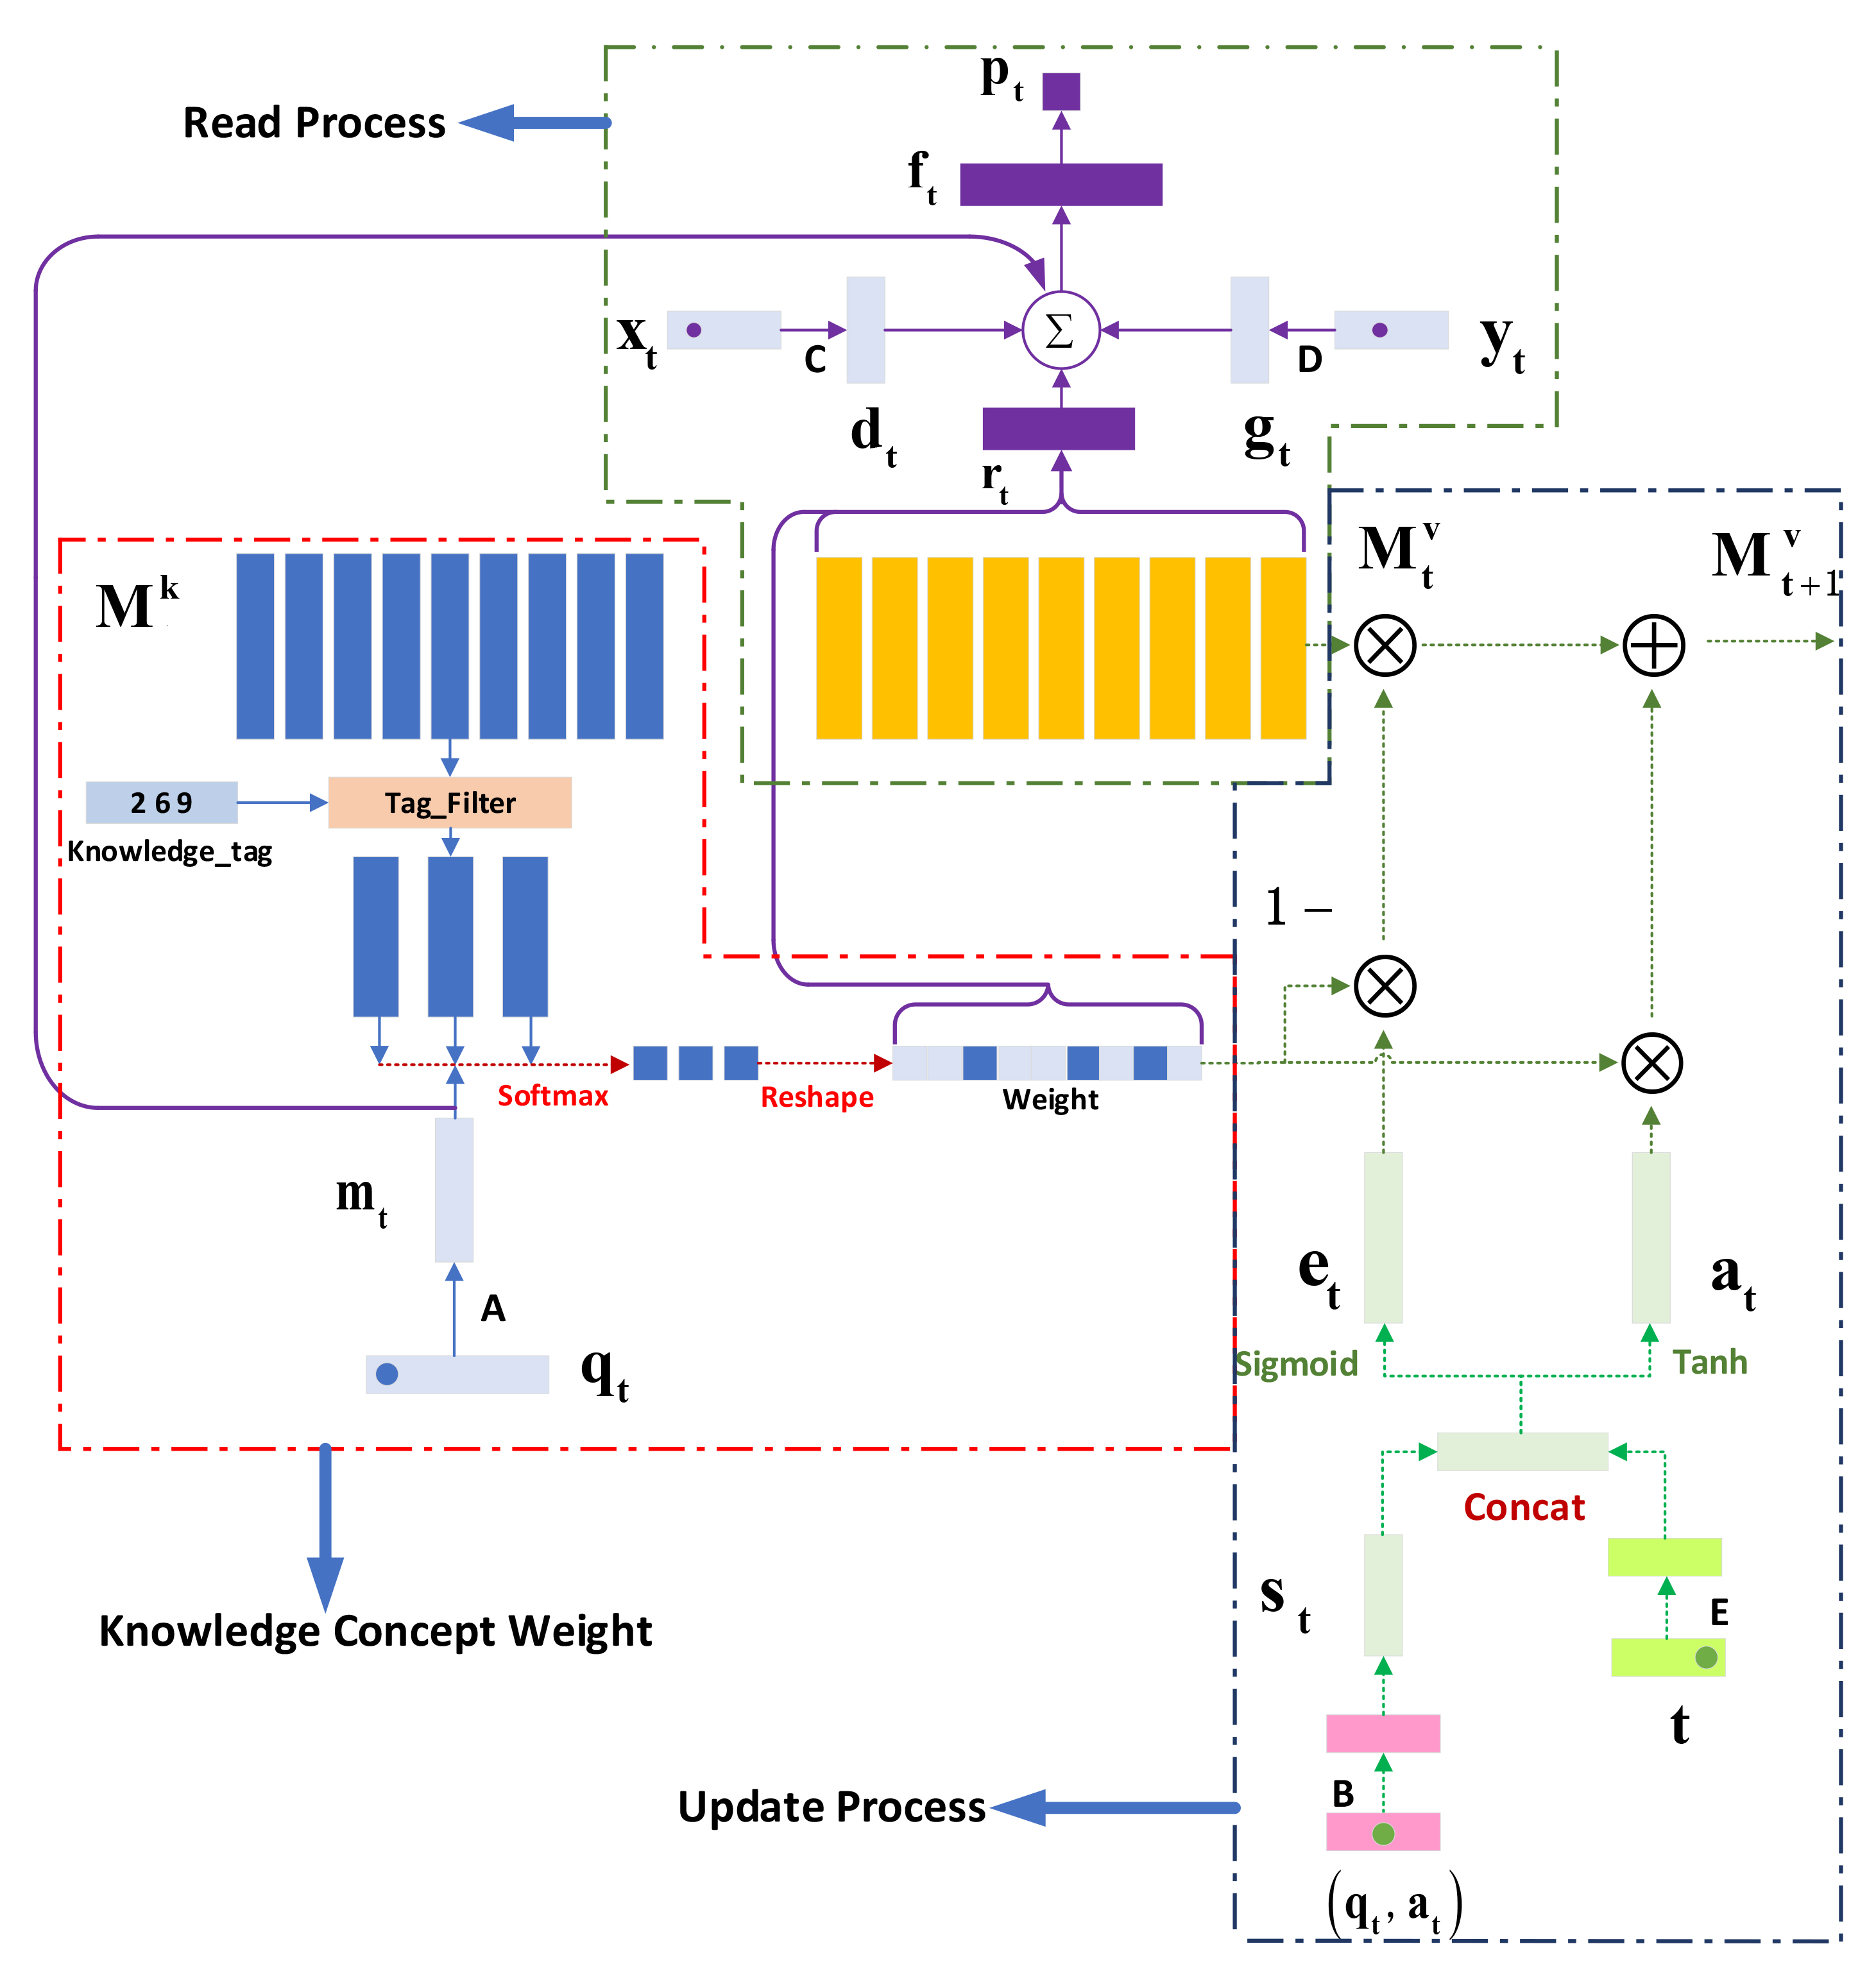
\includegraphics[width=0.5\textwidth]{model.eps}
\caption{Concept-aware DKVMN model structure. }
\label{model}
\end{figure}

We now introduce our knowledge tracing model based on DKVMN model, and highlight our improvement in aspects of memory structure, knowledge concept weight, and read and update process.

\subsection{Concept-Aware Memory Structure}

We modify DKVMN to design its memory structure based on the course's concept list. Fig. \ref{model} plots the model's structure, which is based on DKVMN model\cite{dkvmn}. As shown in Fig. \ref{model}, $\textbf{M}_t^k$ is the concept embedding matrix whose size is $M \times N$, where $N$ is the number of memory locations, and $M$ is the vector size at each location. We set $N$ equal to the number of the course's knowledge concepts. As we have 1 first-level knowledge concept, 7 second-level knowledge concepts and 15 third-level knowledge concepts, we have $N=23$. Then, in each location, the student's state for the corresponding knowledge concept is saved. Thus, the model's memory architecture is explicitly designed to represent knowledge concepts. For comparison, $N$ is a model parameter in DKVMN representing the number of latent knowledge concepts, e.g., $N=5$. As our model is inspired by DKVMN, we name it Concept-Aware DKVMN, i.e., \emph{DKVMN-CA}.

\subsection{Knowledge Concept Weight}

As a student's state of a knowledge concept is saved in the corresponding memory location, when a new exercise arrives, only the exercise's related concepts' memory locations are retrieved and updated. We now present the details of such a procedure. In this section, we calculate the knowledge concept weight (KCW) of the exercise. The weights will be used to calculate the weighted sum of a user's current knowledge concept states to predict her performance on the exercise. It will also be used to update the student's knowledge state after obtaining the answer result of the student on the exercise.

We first obtain the embedding of the arrived exercise.
% Based on DKVMN model structure figure in \cite{dkvmn}, we plot DKVMN-CA structure.
As shown in Fig. \ref{model}, when an exercise $\textbf{q}_t$ arrives at time $t$, it is first transformed into an embedding vector $\textbf{m}_t$ through an exercise embedding matrix $\textbf{A}$. We then calculates the KCW through Algorithm 1. As shown in Algorithm 1,
% the correlation weight is computed by taking the softmax activation of the inner product between $\textbf{m}_t$ and slot \textit{i} of \textit{$M^k_t$} which is corresponding to knowledge tag \textit{i}:}
% \begin{displaymath}
% w_t(i) = Softmax(m_t^TM^k(i)),
% \end{displaymath}
% where $Softmax(z_i)=e^{z_i}/\sum_{j=1}^Ne^{z_j}$.
 % where $Softmax(z_i)=e^{z_i}/\sum_{j=1}^Ne^{z_j}$. Thus, we calculate the three KCWs related to the exercise's three level knowledge concepts, respectively. The KCWs are used for the following read process and update process.
at line 2, we initialize the weight list $R$. As each exercise has three knowledge concepts, the length of $R$ is 3. Then, for each knowledge concept $k$ (line 2), we calculate the dot product of the embedding of the exercise (i.e., $q_t$) and the concept embedding (line 3). We then calculate the KCW by obtaining softmax of $R$, with $Softmax(z_i)=e^{z_i}/\sum_{j=1}^Ne^{z_j}$ (line 6). Then, we initialize an all-zero vector $Weight$ whose length is the number of the knowledge concepts $N$(line 7). For each knowledge concept $k$ of the exercise (line 8), we set its weight value in $Weight$.

In summary, DKVMN computes the relationship weights between the exercise and all latent knowledge concepts, but we just compute the relationship weights between the exercise and its knowledge concepts. For the exercise's relationship weights with other concepts, we set them zeros.
% \emph{Instead of calculating the relationship weights between the exercise and all the latent knowledge concepts like DKVMN, we just calculate the relationship weights between the exercise and its knowledge concepts, as for the relationship weights with the other concepts, we set them with zeros. }

\renewcommand{\algorithmicrequire}{ \textbf{Input:}} %Use Input in the format of Algorithm
\renewcommand{\algorithmicensure}{ \textbf{Output:}} %UseOutput in the format of Algorithm
\begin{algorithm}
\caption{Knowledge Concept Weight Calculation}
\label{alg1} % and a label for \ref{} commands later in the document
\begin{algorithmic}[1]
	\small
	\REQUIRE ~~\\
	$\textbf{q}_t$: embedding of the exercise arrived at time $t$\\
	\textbf{$K_t$}: knowledge concept list of $q_t$\\
	$\textbf{M}^k$: the concept embedding matrix\\

    \ENSURE ~~\\
    $Weight$: Knowledge concept weight of the exercise arrived at time $t$\\
    \vspace{1ex}
    \emph{$/*$ Calculate KCW $*/$} \\
    \STATE $R \Leftarrow [\ ]$
    \FOR{each $n \in$ \textbf{$K_t$}}
    \STATE $corr \Leftarrow \textbf{m}_t^T\cdot\textbf{M}^k[n]$ \\
    \STATE $R.append(corr)$
    \ENDFOR \\
    % % \STATE $Weights \Leftarrow [\ ]$
    \STATE $R_s \Leftarrow Softmax(\emph{R})$ \\
    % % \STATE $Weights \Leftarrow [\ ]$
    % % \FOR{each $\emph{correlation} \in Related$}
    % % \STATE $temp \Leftarrow Softmax(\emph{correlation})$ \\
    % % \STATE $Weights.append(temp)$
    % % \ENDFOR \\
    \vspace{1ex}
    \emph{$/*$ Reshape the weight vector to make its length equal to the number of concepts$*/$} \\
    \STATE $Weight \Leftarrow [0,...,0]$
    \STATE $i \Leftarrow 0$
    \FOR {$i < 3$}
	    \STATE Weight[\textbf{$K_t$}[i]] $\Leftarrow$ $R_s[i]$
	    \STATE $i \Leftarrow i + 1$\\
    \ENDFOR
    \RETURN $Weight$

\end{algorithmic}
\end{algorithm}

\subsection{Read Process}

We then use the obtained KCW to calculate the weighted sum of the user's current knowledge concept states to predict the student's performance on the exercise. Denote KCW by \textbf{w}, we have
% \begin{displaymath}
$\textbf{r}_t = \sum_{i=1}^N\textbf{w}_i\textbf{M}_t^v$, i.e., the knowledge state of concepts related to the exercise \textbf{$q_t$}.
% \end{displaymath}

We further concatenate $\textbf{r}_t$ with the embeddings of the exercise's difficulty and stage feature, i.e., $\textbf{d}_t$ and $\textbf{g}_t$. The result then passes through a fully connected layer with activation function Tanh to get a summary vector $\textbf{f}_t$, which contains all information of the student's knowledge state related to $\textbf{q}_t$ and the exercise's features, i.e.,:
\begin{displaymath}
\textbf{f}_t = Tanh(\textbf{W}_0^T[\textbf{r}_t, \textbf{d}_t, \textbf{g}_t, \textbf{m}_t])
\end{displaymath}
where $Tanh(z_i) = (e^{z_i}-e^{-z_i})/(e^{z_i}+e^{-z_i}).$

Finally, $\textbf{f}_t$ passes through a fully connected layer to output the probability that the student would do the exercises $\textbf{q}_t$ correctly. Denote the probability by \textbf{p}, we have
\begin{displaymath}
\textbf{p} = Sigmoid(\textbf{W}_1^T\textbf{f}_t)
\end{displaymath}
where $Sigmoid(z_i) = 1/(1 + e^{-z_i}).$

\subsection{Update Process}

We then use the KCW to update the student's knowledge state after observing the her answer result. The update process updates the value matrix $\textbf{M}_t^v$, which represents the student's current state of knowledge concept $k$. Our model is different from DKVMN model in that we consider the student's exercising duration in the update process. For comparison, DKVMN ignores this student behavior feature. Specifically, the work in \cite{time} proposed that the a student's duration of solving a problem is related to her master level of latent problem solving skills. Inspired by this work, in our model, after a student finishes an exercise, her answer result (i.e., correct or wrong) $\textbf{a}_t$ and exercising duration are used to update $\textbf{M}_t^v$. Because the exercising duration is a continuous variable, it is firstly discretized according to its distribution and then represented by its embedding \textbf{t}. We then concatenate \textbf{t} with the joint embedding $\textbf{s}_t$ of the answer vector $(\textbf{q}_t,\textbf{a}_t)$, to update $\textbf{M}_t^v$, as shown in Fig. \ref{model}.

The other update process is same as that of DKVMN. It includes erase subprocess and add subprocess. Erase vector is computed as $\textbf{e} = Sigmoid(\textbf{E}^T[\textbf{s}_t,\textbf{t}])$, where \textbf{E} is the erase weights. Add vector is computed as $\textbf{a} = Tanh(\textbf{D}^T[\textbf{s}_t, \textbf{t}])$, where \textbf{D} is the add weights.
 % We consider the exercising duration $\textbf{t}$ for add and erase vector as the exercising time may be related to the growth of the student's knowledge.
% where the shape of \textbf{E} is $(d_t+d_s)*d_v$, the shape of $\textbf{e}$ is $d_v*1$, and each dimension of $\textbf{e}_t$ is in the range (0,1).
Then the new memory matrix $\textbf{M}_{t+1}^v$ is computed by
\begin{displaymath}
\textbf{M}_{t+1}^v(i) = \textbf{M}_t^v(i)[1-\textbf{w}(i)\textbf{e}][1+\textbf{w}(i)\textbf{a}]
\end{displaymath}
% each concept master level vector in $\textbf{M}_t^v$ is erased respectivly according to knowledge related weight.
% then each concept master level vector in $\textbf{M}_t^v$ is added by add vector:
% \begin{displaymath}
% \textbf{M}_{t+1}^v(i) = \textbf{M}_t^v(i)[1+\textbf{w}(i)\textbf{a}]
% \end{displaymath}
% Through the erasing and adding mechanism, the memory matrix $\textbf{M}_t^v$ can be dynamically updated according to features of exercise.
The parameters of the model are learned by minimizing a standard cross entropy loss between the predicted user answer result $p_t$ and her true result $y_t$:
\begin{displaymath}
L = -\sum\limits_{t}((y_tlogp_t) + (1 - y_t)log(1 - p_t))
\end{displaymath}
% The model is trained with Momentum optimization method.\par
In summary, compared with DKVMN, we design the model structure based on the course's concept list, and then explicitly consider the exercise-concept mapping relationship and other exercise's features during students' knowledge tracing.

% we changes the knowledge concepts weight calculation to use the hierarchy knowledge concepts feaures reasonably, and our model considers difficulty and gate feaures to get prediction result, duration feaure to update knowledge state.

\section{Reinforcement Learning Based Exercises Recommendation}

Based on the DKVMN-CA student knowledge tracing model, we build a student simulator which provides environment for reinforcement learning, and train a personalized exercise recommendation agent with deep reinforcement learning method.
% This section introduces our experimental setting.
% \subsection{Exercise Recommendation}

Similar to \cite{acc}, we model the recommendation process as a Partially Observable Markov Decision Process (POMDP), where
% i.e., based on the observation of a student's history of exercise answering result (i.e., correct or wrong), the algorithm decides which exercise should be recommended to the student.
% We model student doing exercises and exercises recommendation as discrete-time, partially-observed Markov Decision process (POMDP).
% A POMDP is described as a set of
the model state is the student's latent knowledge state and the action is the recommendation of an exercise.
% The model transition function $p(s_{t+1}|s_t, a_t)$ means the probability at student's latent knowledge status updating after doing the recommendation exercise $a_t$, and reward function $r(s_t, a_t)$ evaluate the exercise recommended to student at his current latent knowledge status. As for our application,
At time $t$, the reinforcement learning agent cannot observe the student's latent knowledge state $s_t$. Instead, it can observe the student's exercise and answer result (i.e., correct or wrong) $o_t$ which is conditioned on the latent knowledge state $p(o_t|s_t)$. Thus, at time $t$, the agent needs to recommend an exercise $a_t$ based on the student's exercising history before $t$, which is denoted by $h_t$. We have $h_t = (o_1, a_1, o_2, a_2, \dots, o_{t-1}, a_{t-1})$. After the student finishes the recommended exercise $a_t$, her latent knowledge state will turn to $s_{t+1}$ by a transition function $p(s_{t+1}|s_t, a_t)$.
% after the student finishes the recommended exercise $a_t$.
 % which is corresponding to the student doing exercise record $(q_t, an_t)$ where $an_t$ is student's answer correct or not, and observation $o_t$ is conditioned on the underlying knowledge status $p(o_t|s_t)$. So
% Thus, at time $t$, the agent needs to recommend an exercise based on the student's exercising history before $t$, which is denoted by $h_t$. We have $h_t = (o_1, a_1, o_2, a_2, \dots, o_{t-1}, a_{t-1})$. Thus, the agent needs to learn a recommendation policy $\pi(h_t)$ in which it can recommend an exercise  according to $h_t$.

We define the reward $r_t$ of an action $a_t$ as 
\begin{equation}
r_t = \frac{1}{K}\sum\limits_{i=1}^KP_{t+1}(q_i),
\end{equation}
where $K$ is the number of exercises
% whose first-level knowledge concept is "Number Theory"
, and $P_{t+1}(q)$ denotes the probability of the student getting exercise $q$ correct after finishing the recommended exercise at state $s_{t+1}$. It is predicted by the student simulator. So, we name it as the student's \emph{Predicted Knowledge}.
% below: the student's mean probability of getting each exercise correct after finishing the recommended 
% (看下面这个公式,我理解是这样的。但有一点奇怪:难道这个reward不是做了这个action之后学生的平均score的增量,而是现在估计的分数的均值?)
% i.e.,
% \begin{equation}
% r = \frac{\sum\limits_{i=1}^NKS_{t+1}(q_i)}{N}
% \end{equation}
% ~\\
% \centerline{$r = \frac{\sum\limits_{q_i}^NKS_{t+1}(q_i)}{N}$},
% ~\\
% $KS_{t+1}(q)$ means the correct probability in the latent knowledge status of timestamp $t+1$, N is the number of alternative exercises.
% The goal of the agent is thus to learn a recommendation policy $\pi(h_t)$ which make a exercise recommendation according to current student's entire doing exercises history. We want to maximise:\\
% ~\\
% \centerline{$R = \mathbb{E}_{\tau}[\sum\limits_{t=1}^\infty\gamma^{t-1}r(s_t, a_t)]$}
% ~\\
% where trajectories $\tau = (s_1, o_1, a_1, s_2, o_2, a_2, ...)$ are drawn from the trajectory distribution induced by policy $\pi:p(s_1)\\p(o_1|s_1)\pi(a_1|h_1)p(s_2|s_1, a_1)p(o_2|s_2)\pi(a_2|h_2)...$, So we define a deterministic fucntion $a_t = \mu(h_t)$ to represent the policy.
% current student's entire doing exercises history.

The purpose of optimization is to maximize the reward $R$ of policy $\pi$:
\begin{displaymath}
R = \mathbb{E}_{\tau}[\sum\limits_{t=1}^\infty\gamma^{t-1}r(s_t, a_t)],
\end{displaymath}
where trajectories $\tau = (s_1, o_1, a_1, s_2, o_2, a_2, ...)$ are drawn from the trajectory distribution induced by policy $\pi:p(s_1)\\p(o_1|s_1)\pi(a_1|h_1)p(s_2|s_1, a_1)p(o_2|s_2)\pi(a_2|h_2)...$.
Thus, as for the action-value function $Q^\pi$, the reward of the recommended exercise sequence at $t$ is:
\begin{displaymath}
Q^\pi(h_t, a_t) = \mathbb{E}_{s_t|h_t}[r_t(s_t, a_t)] + \mathbb{E}_{\tau > t|h_t, a_t}[\sum\limits_{i=1}^\infty\gamma^ir(s_{t+i}, a_{t+i})]
\end{displaymath}
where $\tau>t=(s_{t+1},o_{t+1},a_{t+1}...)$ is the future trajectory.
% where trajectories $\tau = (s_1, o_1, a_1, s_2, o_2, a_2, ...)$ are drawn from the trajectory distribution induced by policy $\pi:p(s_1)\\p(o_1|s_1)\pi(a_1|h_1)p(s_2|s_1, a_1)p(o_2|s_2)\pi(a_2|h_2)...$,
The algorithm then recommends the exercise $q_{'}$ which has the maximal reward, i.e.,
% . by policy $\pi$ on the basis of student's doing exercises history:
% \begin{displaymath}
$q_{'} = \textbf{max}_aQ^\pi(h_t, a)$.
% \end{displaymath}
% where $h_t$ represents the history of student doing exercises composed of exercise tag and answer status $(q,a)$, $a_t$ represents the recommended exercise at timestamp $t$.
% In summery, we consider the exercises sequence recommendation according to student's entire history of doing exercise as partially-observed Markov Decision process (POMDP), and recommend student the most profitable exercise $q_{'}$ by policy $\pi$ on the basis of student's doing exercises history:
% to student at timestamp $t$.
% \subsection{Recommendation Strategy Optimization}
% The purpose of optimization is to maximize the reward $R$ of policy $\pi$:
% \begin{displaymath}
% R = \mathbb{E}_{\tau}[\sum\limits_{t=1}^\infty\gamma^{t-1}r(s_t, a_t)],
% \end{displaymath}
Similar to \cite{acc}, we approximately solve the POMDP using Trust Region Policy Optimization (TRPO) algorithm \cite{trpo}, with an off-the-shelf implementation from rllab \cite{rllab}.
% \subsection{Experimental Framework}

% Our model training procedure is shown in Algorithm 2. As shown in Algorithm 2, (算法要加行号。然后要逐行解释。), we first initialize the reward. (没看懂). For each epoch, we use (我真的没看懂这个算法在干什么)。
% It first initializes the students' state.

% We then evaluate the model, the Step is 100.

% We first randomly initilize the KT model of a student (line 1).
%  % using her whole historical exercising sequence.
% We first train the recommendation model using TRPO algorithm. Epoch = 100
% For each epoch, we first use the Rllib RL training tool to obtain a sample sequence with current agent (line 7)
% Then, we use TRPO algorithm to update the policy based on the sampling sequence. (line 8)

% The policy is trained by the sample pathes between the agent and environment, we define a student simulator as environment by knowledge tracing model of which the trainable variables have been trained completely and reward function of action is defined in Section 3.1 Eq.1. The optimization algorithm proceeds as presented in Algorithm 2.

% \begin{algorithm}
% \caption{Strategy Optimization Process}
% \label{alg2} % and a label for \ref{} commands later in the document
% \begin{algorithmic}
% 	\small
% 	\REQUIRE ~~\\
% 	\textbf{KS}: The student environment\\
% 	\textbf{Arms}: The alternative recommendation exercise\\
% 	\textbf{Seq}: The history records of student doing exercises of fomat $(q,a)$\\

%     \ENSURE ~~\\
%     The recommendation policy, rewards of each epoch
%     \vspace{1ex} \\
%     \emph{$/*$ Init the student environment by \textbf{Seq} $*/$} \\
%     \STATE $KS.update(\textbf{Seq})$ \\
%     ~\\
%     \emph{$/*$ Sample the pathes and optimize policy $*/$} \\
%     \STATE $t = 0; e = 0; rewards = [\ ]$ \\
%     \WHILE {$e < Epoch$}
% 	    \STATE $pathes\Leftarrow Agent.Parallelizing Sample Process $ \\
% 	    \STATE $Agent.Policy \Leftarrow TRPO(pathes)$ \\
% 	    ~\\
% 	    \emph{$/*$ Evaluate the current policy$*/$} \\
% 	    \STATE $obs \Leftarrow KS.Reset()$ \\
% 	    \FOR {$t < Step$}
% 		    \STATE $action \Leftarrow Agent.Act(obs)$\\
% 		    \STATE $obs, r \Leftarrow KS.Step(action)$\\
% 		    \STATE $rewards.append(r)$ \\
% 		    \STATE $t \Leftarrow t + 1$\\
% 	    \ENDFOR
% 	    \STATE $e \Leftarrow e + 1$
%     \ENDWHILE
%     \RETURN $Agent, rewards$
% \end{algorithmic}
% \end{algorithm}
\section{Performance Evaluation}

In this section, we present the performance evaluation results of our system. 
% of DKVMN-CA knowledge tracing model and the reinforcement learning based exercise recommendation algorithm.

\subsection{DKVMN-CA Knowledge Tracing Model}

We evaluated our model on our IPS dataset. To evaluate it, we conducted 50 experiments. In each experiment, we randomly split the users into two groups: training users and testing users. Their percentages are 70\% and 30\%. We then trained the model with the training users and evaluated the model on the testing users. Similar to \cite{dkt}, we use area under the curve (AUC) as the performance metric. We report the maximal, mean, and the standard deviation of the testing users' AUCs of all 50 experiments.

\subsubsection{Efficiency of Concept-Aware Design}

We first report the efficiency of designing the model's architecture based on the course's knowledge concepts. We compare the performance of DKVMN and DKVMN-CA without the help of other input features, including exercise difficulty, stage, and duration. The results are shown in Table. \ref{addfeature}. See the rows "DKVMN" and "DKVMN-CA". As shown in Table. \ref{addfeature}, our model obtains an AUC of 0.724, which is higher than that of DKVMN model, i.e., AUC = 0.712. Such an improvement is considerable, considering the small improvement DKVMN provides over the DKT baseline (AUC = 0.711). Such a result means that the design of the model's architecture based on the course's knowledge concepts is efficient.

To highlight the necessity of our design, we also evaluate another method which also uses exercises' knowledge concept tags, i.e., represents a knowledge concept by its embedding and then concatenate it with the embedding of the exercise. Its' performance is shown in Table. \ref{addfeature}. See the row "DKVMN-KC". As shown in Table \ref{addfeature}, its mean AUC is 0.714, meaning a very small improvement over the DKVMN (AUC = 0.712). Thus, it is necessary to design the model's architecture based on the course's knowledge concepts to fully utilize their capacity to improve the model.
% We find that the exercises' concept tags indeed cannot bring performance gain to the model, suggesting current practice's rationale.

% We also evaluate the performance of adding the exercise's knowledge concept feature as we add the exercise' difficulty feature(DKVMN+KC in Table. \ref{addfeature}). We find this method only improve a little performance of the DKVMN model.

\subsubsection{Efficiency of Other Exercise Features}

% For comparison, the LSTM model's mean AUC is 71.1\%, meaning the mean AUC of DKVMN model is only 0.1\% higher than the LSTM model in our data. the max AUC of DKVMN-KR model is 72.4\%, which is 1.2\% higher than that of the DKVMN algorithm, meaning

We then evaluate the efficiency of adding other features, including exercise difficulty, stage, and duration. The results are shown in Table \ref{addfeature}. See the rows "DKVMN-CA + Difficulty", "DKVMN-CA + Stage", and "DKVMN-CA + Duration". As shown in Table \ref{addfeature}, these features can further improve the model's performance. For example, the mean AUC of "DKVMN-CA + Stage" is 0.728, which is higher than that of DKVMN model (AUC = 0.712).

% Deep knowledge tracing based on recurrent neural network has made great process. We refer to\cite{hr}, the method of RNN prediction with multi-features, to make our baseline model LSTM\_KG which is a LSTM network with the knowledge concepts type feature.

%As shown in Fig. \ref{beatbaseline}, LSTM and DKVMN have nearly the same performance, KR\_DKVMN perform better than LSTM and LSTM\_KG(1.2\% AUC improvement), but LSTM\_KG has a worse performance than LSTM, this means that the feature needs to be incorporated into the model in a suitable way.

% We second evaluated the efficieny of adding other features. As shown in Table. \ref{addfeature},
% the mean AUCs of DKVMN-KR with features Gate ID is the highest, i.e., 72.8\%, which is 1.6\% higher than that of the DKVMN algorithm.

% We tried to add multiple features and find the model performance cannot exceed that of the DKVMN-KR with Gate feature which also has the most stable performance according to Variance. As for maximum AUCs, DKVMN-KR with features Gate ID and Time is the highest, i.e., 73.9\%,  which is 1.9\% higher than DKVMN algorithm.

% we compare AUC performance of DKVMN, KR\_DKVMN, and models incorporated with other features based on KR\_DKVMN. It's obviously that the difficulty of exercise, the gate where student is doing exercises, the time of finishing exercise, these features all improve the performance of the model to varying degrees. There is 1.9\% AUC improvement compared with baseline model DKVMN. Among them, the feature of knowledge concepts is the most effective to improve the performance which is 1.2\% AUC improvement.

\begin{table}
\centering
\caption{AUC of Models with Different Features}
\label{addfeature}
\begin{tabular}{|p{2.3cm}|c|c|c|} \hline
Model&Mean AUC&Max AUC&Variance\\ \hline
LSTM & 0.711 & 0.712 & 1.86e-05\\ \hline
DKVMN & 0.712& 0.720 & 2.05e-05\\ \hline
DKVMN-KC & 0.714& 0.724 & 1.85e-05\\ \hline
DKVMN-CA& 0.724& 0.731 & 2.14e-05\\ \hline
DKVMN-CA + Stage & \textbf{0.728}& 0.736 & \textbf{1.48e-05}\\ \hline
DKVMN-CA + Duration & 0.725& 0.737 & 1.75e-05\\ \hline
DKVMN-CA + Difficulty & 0.726& 0.736 & 2.44e-05\\ \hline
DKVMN-CA + Stage, Duration& 0.726& \textbf{0.739} & 2.43e-05\\ \hline
% $+$All Above & 0.726& 0.737 & 1.91e-05\\ \hline
\end{tabular}
\end{table}

% In summery, we detect by experiments on real education data that features of exercises and student's behaviors characteristics all improve the performance of knowledge tracing to varying degrees. Especially, knowledge points of exercises are important to knowledge tracing, our model KR\_DKVMN with gate feature gets the best performance which is AUC 1.9\% higher than baseline models.

% \begin{figure}
% % \centering
% \includegraphics[width=0.5\textwidth]{beatbaseline.pdf}
% \caption{AUC of Models}
% \label{beatbaseline}
% \end{figure}

\subsection{Exercises Recommendation}

% Based on our DKVMN-KR model, we built a student simulator, which is able to trace a student's knowledge status during her exercising process and predict the result (i.e., correct or wrong) of the next exercise. We
% model student doing exercises and exercises recommendation as discrete-time, partially-observed Markov Decision process, and optimize the
% learn the recommendation policy by reinfor algorithm. We name this policy as \textbf{RL policy}. First, we initialize the student simulator randomly, and train the agent 100 epoches. Each epoch we evaluate the policy by mean value of 30 steps'rewards. As shown in Fig. \ref{trpo}, as the number of training epoch increases, the policy performs better and better, mean value of rewards increases from 74\% to 90\%.

% \begin{figure}
% % \centering
% \includegraphics[width=0.5\textwidth]{trpo.eps}
% \caption{Strategy Evaluation}
% \label{trpo}
% \end{figure}

% This subsection presents the performance of our exercise recommendation algorithm obtained by reinforcement learning.

\subsubsection{Evaluation of Students' Knowledge Growth Process}

We use the Expectimax algorithm proposed in \cite{dkt} as the baseline algorithm. In the Expectimax algorithm, the system first calculates a student's predicted knowledge assuming an exercise is recommended to the user to practice. It then chooses the exercise with the highest predicted knowledge to recommend.
% \cite{dkt} propose that choosing the entire sequence of next exercises so as to maximize predicted accuracy can be phrased as a Markov decision problem, and can also evaluate the benefits of using

To compare the two algorithms, we first randomly pick 15 students in our dataset. For each student, we conduct two experiments, one experiment for one algorithm. In each experiment, we first initialize the student simulator using the student's historical practice sequence. Then, we continuously recommend 50 exercises to the student simulator with the recommendation algorithm. During the process, we record the average of the 15 students' predicted knowledge as Eq.(1) at each step of recommendation. The results are shown in Fig. \ref{compare}. As shown in Fig. \ref{compare}, the students served by RL policy has a higher mean predicted knowledge than the students served by the Expectimax policy after 50 exercises. Moreover, after about 10 exercises, the mean predicted knowledge of the students served by the Expectimax policy stops increasing, meaning that the policy cannot find exercises which can help the students to improve the performance any more. For comparison, served by the RL policy which considers long-term reward of action, the students' mean predicted knowledge keeps increasing, meaning that the RL policy still can find exercises which can help the student to improve performance.
% , while the increasing rate is slow as the predicted knowledge is close to 1, i.e., the perfect score.

% the 50 timestamps recommendation, the performance of RL policy is 5\% higher than Expectimax policy, and has a rising trend. But as for Therefore, RL policy is more suitable for exercise sequence recommendation.

\begin{figure}
% \centering
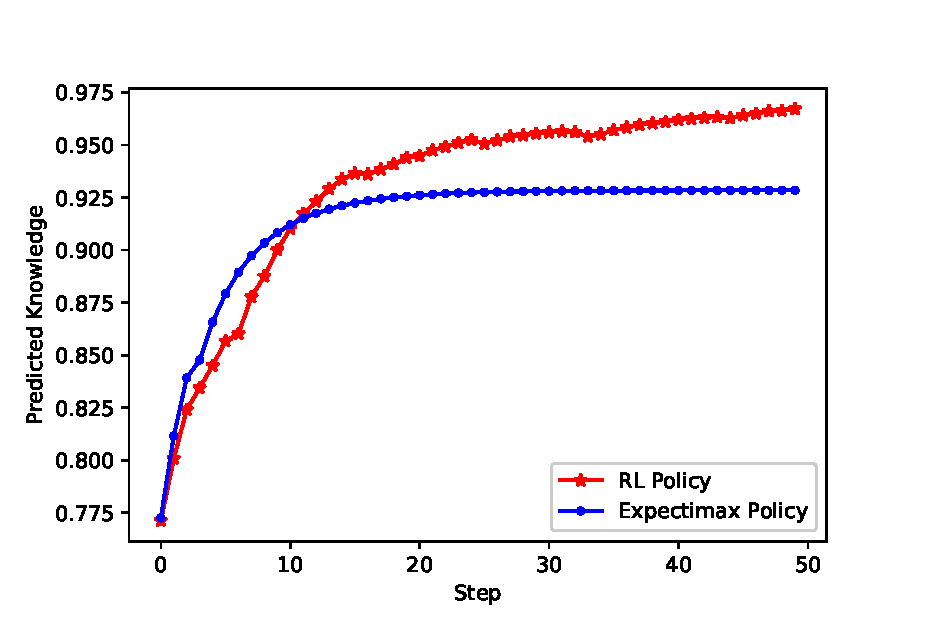
\includegraphics[width=0.5\textwidth]{predicted_knowledge.eps}
\caption{Performance evaluation results}
\label{compare}
\end{figure}

\subsubsection{Evaluation of Recommendation Process}

We design another experiment to observe the recommendation behavior of the RL policy. We randomly pick a student who has practiced five exercises, and use her exercise sequence to initialize the student simulator. Then, we serve her with five more exercises using the RL recommendation policy. Fig. \ref{recom} shows the results. The x label of Fig. \ref{recom} shows the 10 exercises' IDs, concepts, and results. For example, the first record (88, 5, 0) means that the exercise ID is 88, which is related to concept 5, and the student's answer is wrong. As the 10 exercises are related to 6 concepts, we plot the student's predicted knowledge of each concept in Fig. \ref{recom}. For instance, as the student fails in the first exercise 88, which is related to the 5th concept, the student's knowledge status on the 5th concept is relatively low. The status of the knowledge concepts not covered by the student's history exercises are indicated in black. We now observe the recommended exercises. We have the following observations:

\begin{figure}
% \centering
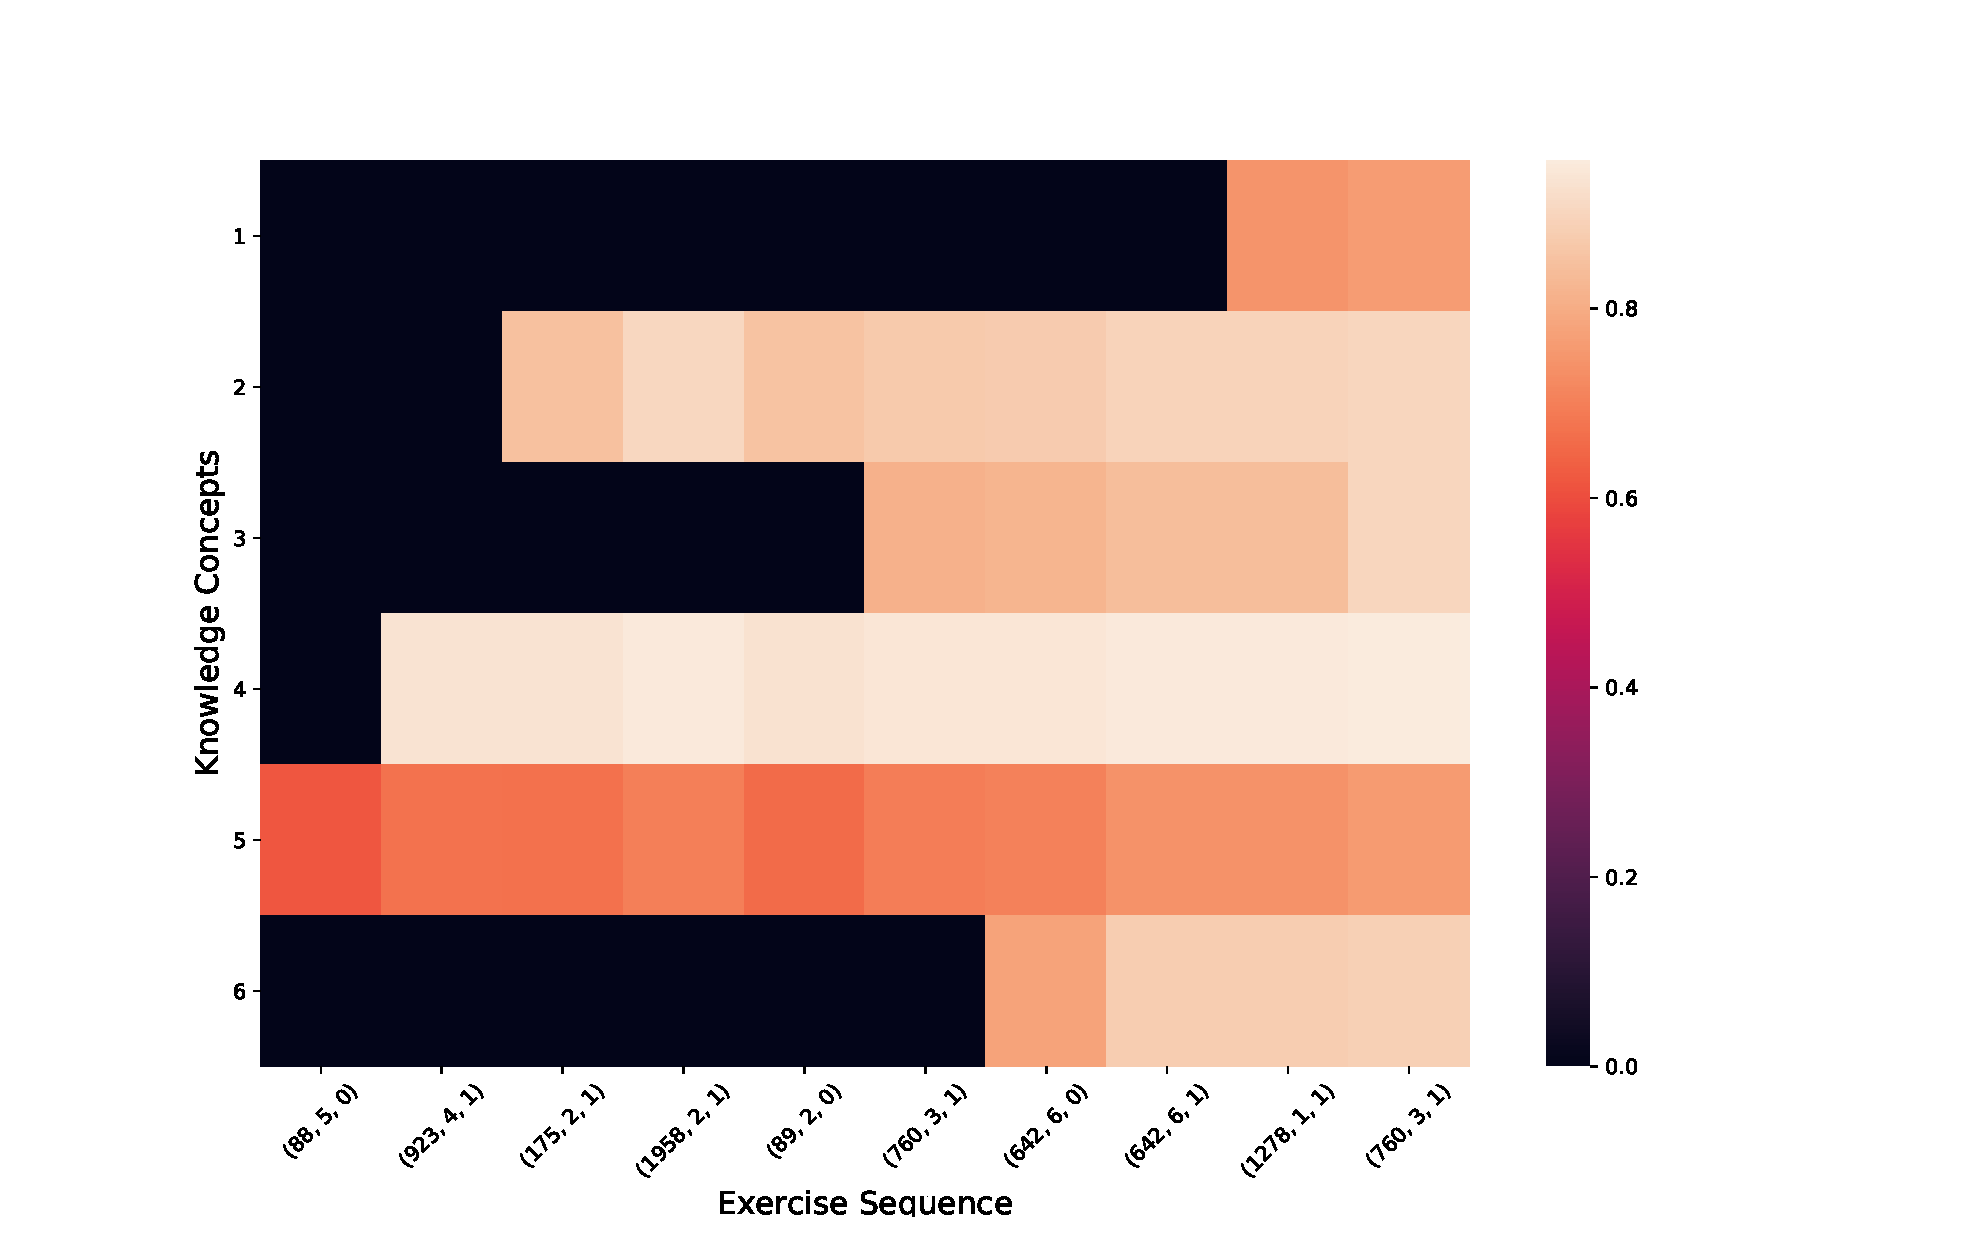
\includegraphics[width=0.55\textwidth]{recom1.eps}
% 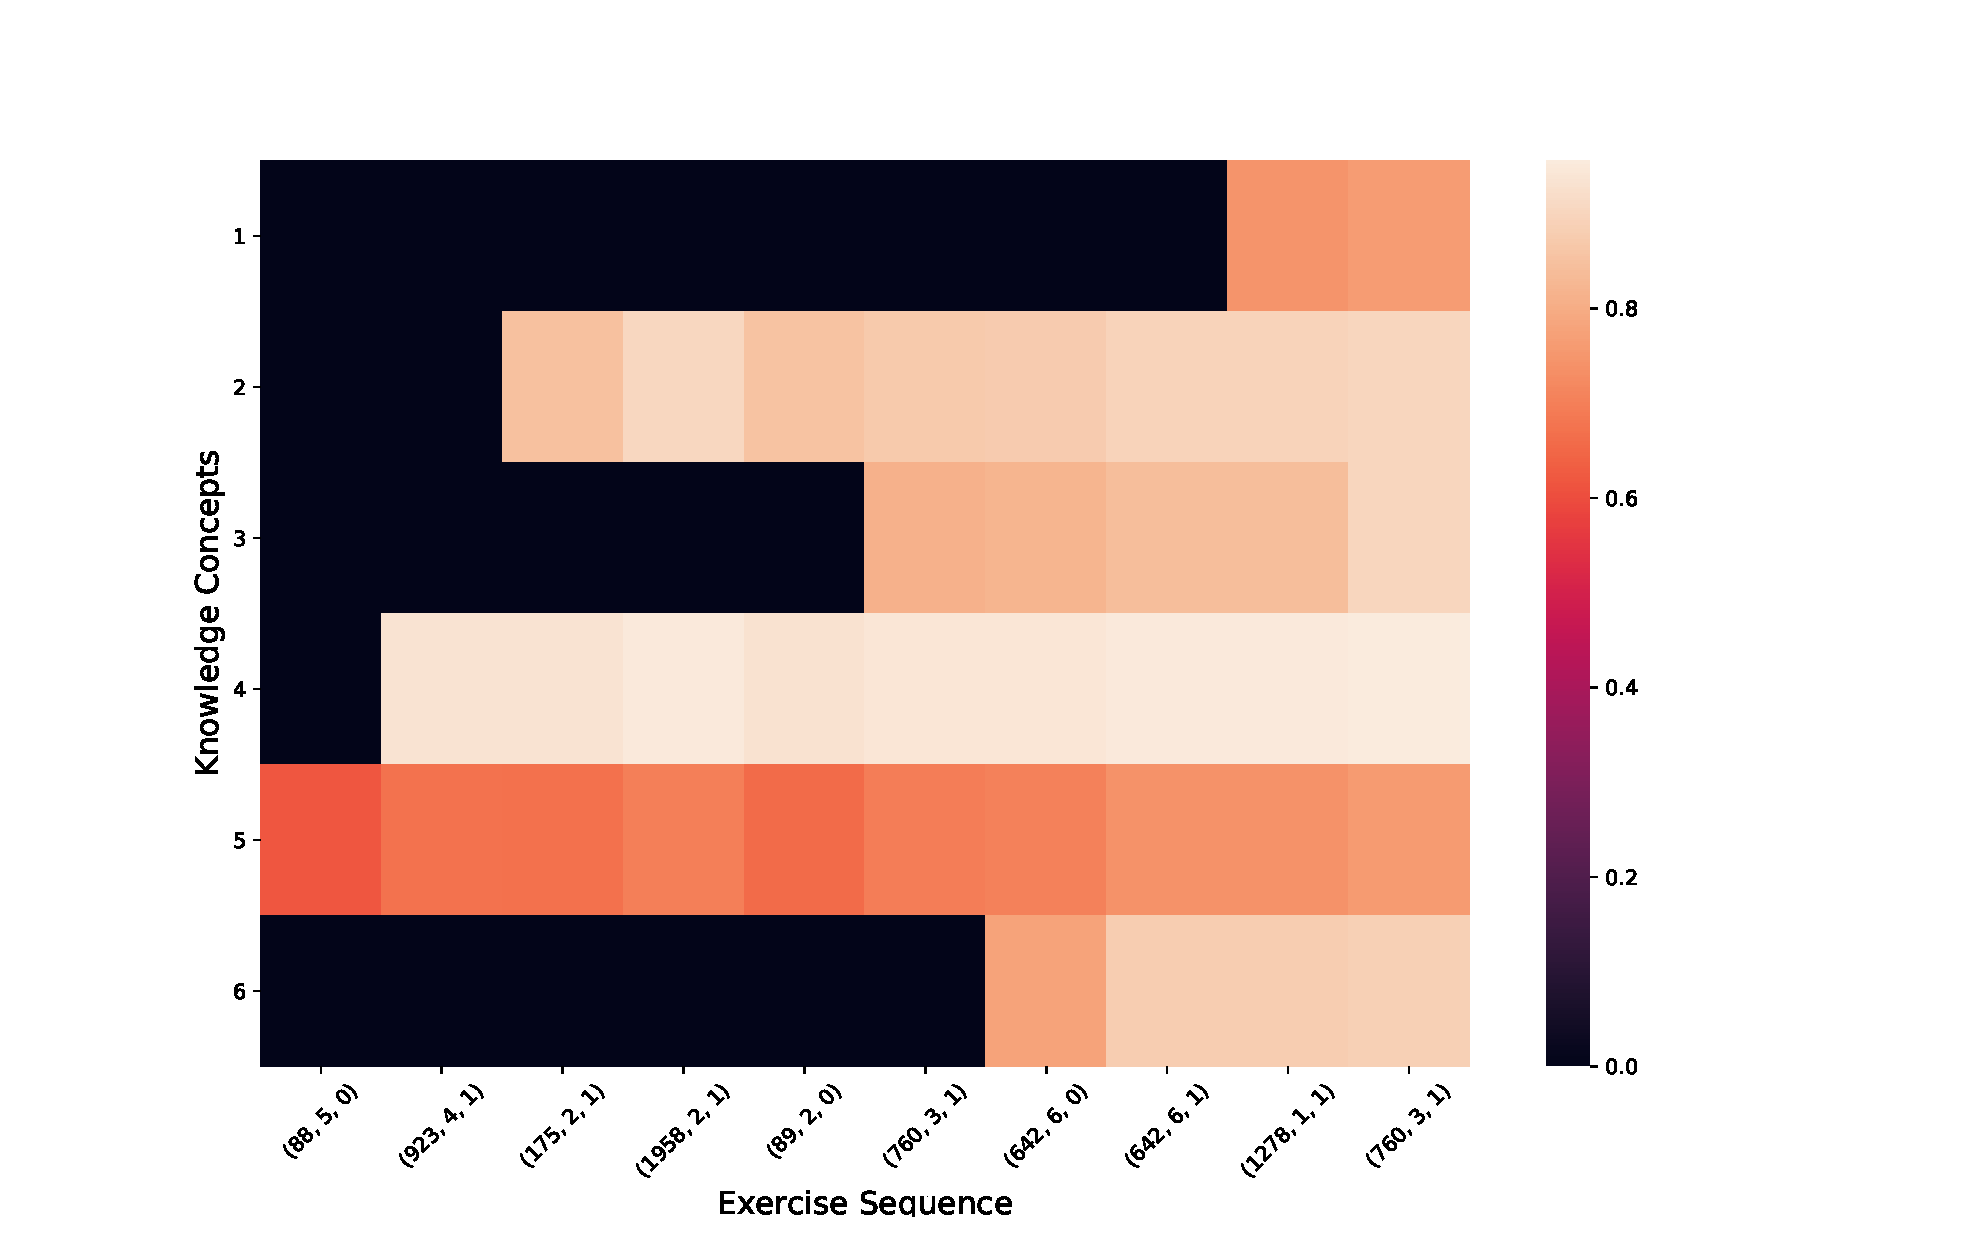
\includegraphics[width=8cm, height=5cm]{recom1.eps}
\caption{Knowledge State Variation}
\label{recom}
\end{figure}

% 5,4,2,2,2,3,6,6,1,3


\begin{itemize}
	\item As shown in Fig. \ref{recom}, the first five exercises are related to concepts {2,4,5}, and the later five exercises are related to concepts {1,3,6}, suggesting the RL algorithm wants to explore the student's capacity in other concepts.
	\item After the student succeeds in exercise 760, which is related to the concept 3 (Decomposition of Prime Factor), the algorithm recommends the exercise 642, which is related to concept 6 (Maximum common factor and Least common multiple). As concept 6 is related to concept 3, such a recommendation is reasonable.
	\item The student, however, fails to finish the exercise 642. Thus, the algorithm recommends exercise 642 again. This time, the student succeeds to finish it, meaning that the model captures the phenomenon during training that a student who failed in exercise 642 may succeed if she retries. Such a result is interesting.
	\item After the student succeeds in exercise 642, which is related to concept 6 (Maximum common factor and Least common multiple), the model's estimation of the student's capacity on concept 3 (Decomposition of Prime Factor)also slightly increases. As these two concepts are indeed related, such a result is reasonable.
	\item Then, the algorithm turns to another concept again, i.e., it recommends the exercise 1278, which is related to concept 1. While the student succeeds in the exercises, the estimated student's knowledge status on the concept 1, however, is relatively low, suggesting that the exercise is relative easy.
	\item At last, the exercise 760 is recommended again, and the student succeeds in it. As a result, the model's estimation of the student's capacity on concept 3 increases, suggesting that reviewing is beneficial for study.
\end{itemize}

% another plots the visualize the variation of knowledge status as the student is served by RL recommendation policy.

% As shown in Fig. \ref{recom}, a color patch represents the average of probability answering exercises correctly of the same knowledge point. The status of the knowledge points not covered by the student's history exercises is indicated in black.

% The first five records are history of student exercised involving 2,4,5 knowledge points, and the last five exercises are recommended by RL policy. In order to improve each knowledge points master level, the policy recommends the exercises not only involving 2,4,5 knowledge points, but also the other dependence knowledge points. For example, this student did not answer the exercise of \textit{Same Reminder} knowledge point correctly, it recommends the exercises of it's basic knowledge point \textit{Decomposition Prime Factor}. As the student do the following recommended exercises, student gets improvement on all 2,4,5 knowledge points.

% In summary, we model the exercises sequence recommendation as POMDP, and optimize the policy by TRPO algorithm. The policy performs better on exercises sequence recommendation than expectimax algorithm based on MDP search, and considers the relationship between different knowledge points.

\section{conclusion}

In this paper, we improve DKVMN by designing its neural network structure based on a course's concept list, and explicitly considering the exercise-concept mapping relationship during students' knowledge tracing. We also enhance the DKVMN model to consider more input features. Experimental results show that our model has higher performance than existing deep knowledge tracing models. We also propose an exercises recommendation algorithm which uses model-free reinforcement learning with neural network function approximation to learn an exercise recommendation policy that directly operates on raw observations of a student's exercise history.
Our experimental results demonstrate that our policy achieves better performance than existing heuristic policy in terms of maximizing the students' knowledge level. To the best of our knowledge, this is the first time that deep reinforcement learning has been applied to personalized mathematic exercise recommendation.
 % Experimental results shown that with the help of the policy, students have higher predicted knowledge after solving fewer problems. To the best of our knowledge, this is the first time that deep reinforcement learning is applied for personalized mathematic exercise recommendation.

% In this paper, we apply exercise features and student's behavior characteristics to knowledge tracing, improve the performance of knowledge tracing model based on Dynamic Key-Value Memory Network, and we detect that knowledge points of exercise are really important to knowledge tracing. Then we build a student simulator based on our improved model which can dynamically update the knowledge status during doing exercises, through this student simulator, we proposes a exercises sequence recommendation algorithm based on POMDP, and optimize the policy by TRPO algorithm, the policy can recommend student exercises to learn according to history answer results of exercises. Instead of considering expectimax the benefits of next step, it paies attention to long-term benefit of each recommendation, so it is more suitable for exercises sequence recommendation. Based on real exercises records of students, we compare our recommendation policy with baseline algorithm and achieve better or comparable performance than baseline algorithm.
% \emph{There are a number of avenues for future work. First, deep representation of exercise is important for knowledge tracing, we will consider exercise' semantic feature to rebuild the representation of exercise, and build the deep representation of massive exercises data by similar exercises algorithm. Second, we will consider knowledge graph to optimize our policy, let our policy more personalized and explainable.}
% \begin{thebibliography}{00}

% \end{thebibliography}

% \section{}
\section{Acknowledgement}
This work was supported by National Natural Science Foundation of China under Grants 61572071, 61872031, and 61301082.

\bibliographystyle{abbrv}
\bibliography{refer}

% \begin{thebibliography}{00}

% \bibitem{dkt} Chris Piech, Jonathan Bassen, Jonathan Huang, Surya Ganguli, Mehran Sahami, Leonidas J Guibas, and Jascha Sohl-Dickstein. Deep knowledge tracing. \textit{In Advances in Neural Information Processing Systems}, pages 505–513, 2015.
% \bibitem{dkvmn} Jiani Zhang, Xingjian Shi, Irwin King, Dit-Yan Yeung. Dynamic Key-Value Memory Networks for Knowledge Tracing. \textit{the 26th International Conference on World Wide Web}, 2017
% \bibitem{bkt} Albert T Corbett and John R Anderson. Knowledge tracing: Modeling the acquisition of procedural knowledge. \textit{Conference on User modeling and user-adapted interaction}, 4(4):253–278, 1994.
% \bibitem{hdd} Mohammad Khajah, Robert V Lindsey, and Michael C Mozer. How deep is knowledge tracing? \textit{arXiv preprint arXiv:1604.02416}, 2016.
% \bibitem{ees} Yu Su, Qingwen Liu, Qi Liu, Zhenya Huang. Exercise-Enhanced Sequential Modeling for Student Performance Prediction. \textit{The Thirty-Second AAAI Conference on Artificial Intelligence}, 2018.
% \bibitem{zpd} IA Chounta, BM McLaren, PL Albacete, PW Jordan. Modeling the Zone of Proximal Development with a Computational Approach. \textit{Conference on Educational Data Mining}, 2017.
% \bibitem{mab} B Clement, D Roy, PY Oudeyer, M Lopes. Multi-armed bandits for intelligent tutoring systems. \textit{Conference on Educational Data Mining}, 2015.
% \bibitem{ucb} AS Lan, RG Baraniuk. A Contextual Bandits Framework for Personalized Learning Action Selection. \textit{Conference on Educational Data Mining}, 2016.
% \bibitem{acc} Siddharth Reddy, Sergey Levine, and Anca Dragan. Accelerating Human Learning with Deep Reinforcement Learning. \textit{NIPS'17
% Workshop: Teaching Machines, Robots, and Humans}, 2017.
% \bibitem{trpo} John Schulman, Sergey Levine, Pieter Abbeel, Michael Jordan, and Philipp Moritz. Trust region policy optimization. \textit{ICML'15}, 2015.
% \bibitem{rllab} Yan Duan, Xi Chen, Rein Houthooft, John Schulman, and Pieter Abbeel. Benchmarking deep reinforcement learning for continuous control. \textit{ICML'16}, 2016.
% \bibitem{hr} Rajkomar A , Oren E , Chen K , et al. Scalable and accurate deep learning with electronic health records. \textit{npj Digital Medicine}, 2018, 1(1):18.
% \bibitem{time} Pelánek, Radek, Jarušek, Petr. Student Modeling Based on Problem Solving Times. \textit{J.Artificial Intelligence in Education}, 25.4(2015):493-519.





% \end{thebibliography}

\end{document}